%!TEX root = cvl_bachelor_thesis.tex

%-------------------------------------------------------
% Results
%-------------------------------------------------------
\section{Results}
\label{sec:results}

%----------------------------------------------
% * Geschwindigkeit 
%----------------------------------------------
\subsection{Performance}
\label{sec:Performance}

In Absatz \ref{sec:Berehnung_der_Fensterung} wurden zwei Ansätze zur Berechnung der Fensterung vorgestellt,
welche jeweils auf unterschiedlichen vom Browser zur Verfügung gestellten API's basieren.
In diesem Unterkapitel wird gezeigt, wie sich diese beiden Verfahren im Bezug auf ihre Performance verhalten.
Dazu wird ein Testsystem vorgestellt, mit dem diese gemessen wurde und weiters werden die Ergebnisse dieser Messungen präsentiert und diskutiert.

\subsubsection{Messverfahren}
Um zu evaluieren wie performant ein Verfahren ist,
wurde über einen bestimmten Zeitraum $T_m$ ermittelt, wie viele Bilder durchschnittlich in der Sekunde berechnet werden können.
Dieser Wert wird als Framerate bezeichnet und in FPS (Frames per Second) angegeben.
Die Framerate ist von folgenden Faktoren abhängig:
\begin{itemize}
	\item Berechnungs-Verfahren
	\item Anzahl der Pixel im Bild
	\item Verwendete Hardware
	\item Verwendeter Browser
	\item Aktuelle Auslastung der Maschine
\end{itemize}
Die ersten vier Parameter wurden für die verschiedenen Messungen variiert, während der letzte eine Störgröße darstellt, welche nur bedingt beeinflusst und nicht absolut konstant gehalten werden kann.
Bei jeder Messung wurden die durchschnittlichen FPS in Abhängigkeit von der Bildgröße aufgenommen.
Eine Messung besteht daher aus einer Menge von Messpunkten, wobei jeder die durchschnittliche Framerate für eine bestimmte Bildgröße angibt.
Dabei wurde ein quadratisches Bild verwendet und dessen Kantenlänge zwischen zwei Messpunkten jeweils um einen bestimmten Wert $\Delta_{edge}$ vergrößert.
Die Pixelanzahl zwischen zwei Messpunkten hat somit ein quadratisches Wachstum wie es auch beim Zoomen von Bildern in der Applikation der Fall ist.

Für die Durchführung der Messung wurde eine eigene Messumgebung entwickelt, 
mit welcher es möglich ist die Implementierung der beiden Verfahren mit unterschiedlichen Parametern zu testen.
Die Messumgebung besteht aus einem Servlet welches mit Spring MVC implementiert wurde und aus einer Clientseitigen Testumgebung für die Implementierungen der beiden Verfahren.
Eine Messung wird durch den Aufruf einer Resource auf dem Servlet gestartet und parametriert.
Das Servlet retourniert darauf hin eine Webseite in welcher die Testumgebung als JavaScript ausgeführt wird.
Diese versucht auf einem Bild die Fensterung mit einer Ziel-Framerate von 60FPS zu berechnen und misst Abfälle in der Framerate.
Für die eigentliche Messung wurde das Tool Stats.JS verwendet und geringfügig modifiziert um die gemessenen Werte auslesen zu können.
Nach Ablauf der Messzeit $T_m$ werden die gemessenen Werte zurück an den Server gesendet, welcher diese in eine Datenbank schreibt.
Der Server antwortet darauf mit einem neuen Messpunkt wobei das Testbild zwischen den Messpunkten jedes mal um den Wert $\Delta_{edge}$ vergrößert wird, 
bis es eine vorher festgelegte maximale Bildgröße ereicht hat.

\subsubsection{Ergebnisse}
Im letzten Unterkapitel wurde ein Verfahren zur Ermittlung der Framerate in Abhängigkeit von der Bildgröße vorgestellt, 
sowie mehrere Parameter welche auf diese Größe einen Einfluss haben.
Von diesen Parametern wurden die Hardware \ref{tab:tested_hardware}, 
der Browser \ref{tab:tested_browser} und das Verfahren zum Rendern \ref{tab:tested_technologies} in unterschiedlichen Kombinationen getestet und einen Kennline ermittelt.
\begin{figure}[t]
	\centering
	\begin{tabular}{| l | l | l |}
		\hline
				& PC				& Tablet \\
		\hline
		Prozessor	& Intel Core i7-2600K 3.40GHz	& Nvidia Tegra 3 1.30GHz \\
		Arbeitsspeicher	& 12GB DDR3-1333		& 1GB DDR3-1333 \\
		Grafikkarte	& Nvidia GeForce 8800 GTS	& Nvidia GeForce ULP \\
		GPU Kerne	& 96				& 12 \\
		Grafikspeicher	& 640MB 800 MHz			& Shared mit CPU \\
		Betriebssystem	& Windows 8			& Android 4.4.4 \\
		\hline
	\end{tabular}
	\caption{Harware-Konfiguration der geteseten Geräte}
	\label{tab:tested_hardware}
\end{figure}
\begin{figure}[t]
	\centering
	\begin{tabular}{| l | l |}
		\hline
		Browser			& Version \\
		\hline
		Chrome			& 39.0 \\
		Chrome for Android 	& 39.0 \\
		FireFox			& 34.0.5 \\
		InternetExplorer	& 11.0 \\
		Opera			& 26.0 \\
		Safari			& 5.1.7 \\
		\hline
	\end{tabular}
	\caption{Getestete Browser}
	\label{tab:tested_browser}
\end{figure}
\begin{figure}[t]
	\centering
	\begin{tabular}{| l | l |}
		\hline
		Verfahren	& Verwendete Technologien \\
		\hline
		WebGL		& Canvas3D API, Pixi.JS, JavaScript \\
		Canvas 2D	& Canvas2D API, JavaScript \\
		\hline
	\end{tabular}
	\caption{Getestete Verfahren mit verwendeten Technologien}
	\label{tab:tested_technologies}
\end{figure}


Die Abbildungen \ref{fig:stat_renderer_pc_chorme} und \ref{fig:stat_renderer_tablet_chorme} zeigen einen Vergleich der beiden rendering Verfahren auf jeweils unterschiedlicher Hardware mit Chrome.
In beiden Fällen verhält sich WebGl wesentlich performanter als das Rendering der Bilder in der CPU.
Am PC mit einer Grafikkarte aus dem Jahr 2007 wurden Bilder bis zu 3000Pixel Kantelänge getestet, 
welche sich ohne Einbrüche mit 60FPS render liesen.
Dieses Verhalten lässt sich dadurch erklären dass eine GPU für diese Anwendung wesentlich geeigneter ist.
Zu den beschleunigenden Faktoren zählen unter anderem, das Zusammenarbeiten vieler paralleler Shader-Kerne welche selbst wiederum sehr stark für diese Art von Berechnungen optimiert sind.
Weitere Faktoren sind die schnelle Anbindung des Grafikspeichers in dem das Bild als Textur abgelegt wird, und dass die GPU auf weniger parallele Prozesse aufgeteilt wird als die CPU.
Am PC wurden dieses Tests auch mit anderen Browsern durchgeführt welche hier nicht abgebildet sind, da die Ergebnisse sehr ähnlich waren.

Unterschiede zwischen den verschiedenen Browsern zeigten sich nur beim Rendern mit Canvas 2D was in Abbildung \ref{fig:stat_browser_js_pc} dargestellt wird.
Bei dieser Gegenüberstellung wird die Performance ausschließlich durch die Implementierung des Browsers bestimmt,
wobei hier die Effizienz der JavaScript-Engine am meisten Einfluss hat.
Bei diesen Test ist noch anzumerken dass nicht davon ausgegangen werden kann, 
dass die JavaScript Interpreter für diese Art von Operationen, 
also dem verarbeiten von großen linearen Daten-Arrays optimiert wurden, 
da diese Art der Datenverarbeitung in klassischen Html5 Anwendungen eher selten vorkommt.
Das unterschiedliche Verhalten der Browser mit WebGl wurde hier nicht dargestellt da die Performance bis zu einer Größe von 3000Pixel Kantenlänge bei allen Browsern konstant 60FPS beträgt.
Die einzige Ausnahme bildet der Browser Safari in welchen WebGl nur experimentell verfügbar ist und extra aktiviert werden muss, was in der getesteten Version nicht möglich war.
Es ist auch anzunehmen dass beim Rendern mit WebGl der Browser selbst keine nennenswerte Rolle spielt da die Datenverarbeitung in der GPU passiert und der Browser nur das Ergebnis darstellt.

In den Abbildungen \ref{fig:stat_hardware_js_chrome} und \ref{fig:stat_hardware_webgl_chrome} wird die Performance auf unterschiedlicher Hardware gezeigt.
Obwohl sich beim Browser Chrome die Tablet Version in einigen Features von der Desktop Version unterscheidet, 
ist anzunehmen dass Dies auf die Performance keine Auswirkung hat da sie beide die selbe JavaScript Engine verwenden.
Die Unterschiede in der Leistung beim Rendern mit Canvas 2D erklärt sich durch die wesentlich geringere Leistung der CPU im Tablet gegenüber dem PC.
Beim Rendern mit WegGl führt die schwächere GPU des Tablets zu der schlechteren Performance.

\begin{figure}[pt]
	\centering
	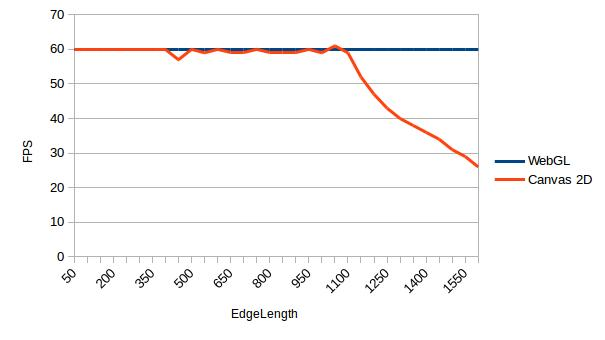
\includegraphics[width=0.7\linewidth]{img/c4_stat_renderer_pc_chorme.jpg}
	\caption{Performance unterschiedlicher rendering Verfahren am PC mit Chrome}
	\label{fig:stat_renderer_pc_chorme}
\end{figure}

\begin{figure}[pt]
	\centering
	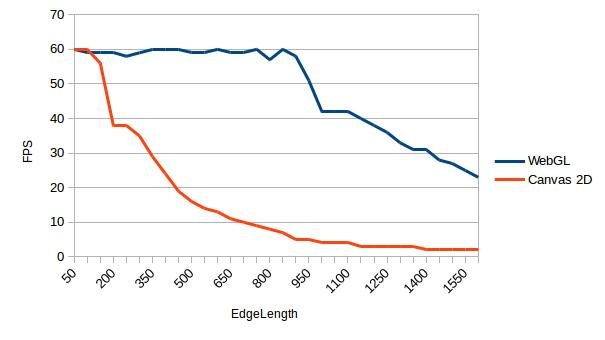
\includegraphics[width=0.7\linewidth]{img/c4_stat_renderer_tablet_chorme.jpg}
	\caption{Performance unterschiedliche rendering Verfahren am Tablet mit Chrome}
	\label{fig:stat_renderer_tablet_chorme}
\end{figure}

\begin{figure}[pt]
	\centering
	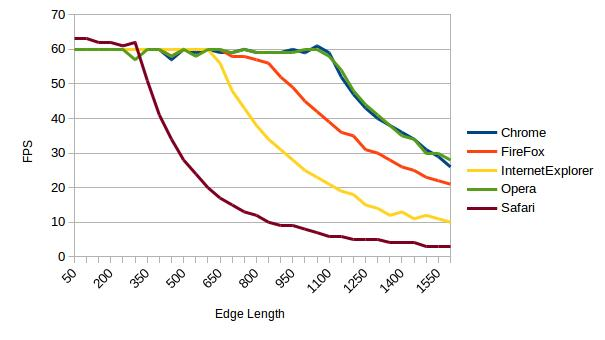
\includegraphics[width=0.7\linewidth]{img/c4_stat_browser_js_pc.jpg}
	\caption{Performance unterschiedlicher Browser beim Rendering mit Canvas 2D}
	\label{fig:stat_browser_js_pc}
\end{figure}

\begin{figure}[pt]
	\centering
	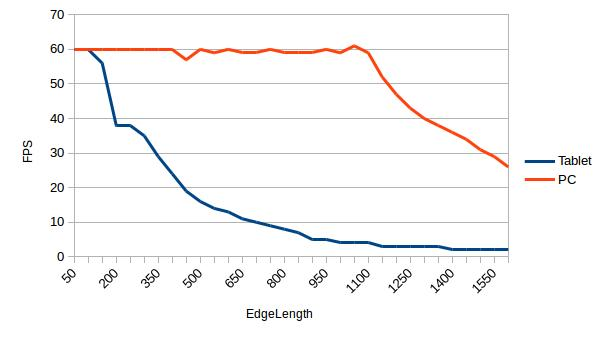
\includegraphics[width=0.7\linewidth]{img/c4_stat_hardware_js_chrome.jpg}
	\caption{Performance unterschiedlicher Hardware mit Canvas 2D in Chrome}
	\label{fig:stat_hardware_js_chrome}
\end{figure}

\begin{figure}[pt]
	\centering
	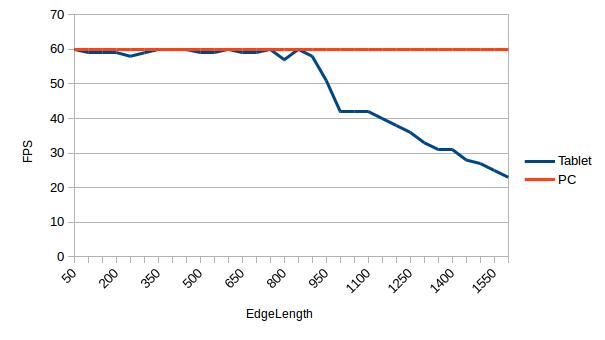
\includegraphics[width=0.7\linewidth]{img/c4_stat_hardware_webgl_chrome.jpg}
	\caption{Performance unterschiedlicher Hardware mit WebGL in Chrome}
	\label{fig:stat_hardware_webgl_chrome}
\end{figure}

\subsubsection{Zusammenfassug der Ergebnisse}
Im letzten Unterkapitel wurden Messergebnisse für die Performance in Abhängigkeit von Rendering-Verfahren, Hardware und Browser gezeigt.
Zusammenfassen lässt sich sagen, 
dass unter der Verwendung von WebGl auf einem aktuellen PC, 
Bilder bis zu einer Auflösung von 9 MegaPixel problemlos fenstern lassen.
Auf dem verwendeten Tablet liegt die Grenze bei ca einem MegaPixel.
Rendern mit Canvas 2D liefert im Vergleich zu WebGl wesentlich schlechtere Performance und lässt sich in der Praxis am Tablet nicht sinnvoll verwenden.


%----------------------------------------------
% * Usability
%----------------------------------------------
\subsection{Vergleich mit dem KRESHMOI JavaClient}
\label{sec:Usability}
In der Einführung wurde bereits erwähnt, 
dass für KRESHMOI parallel zu der in diesem Projekt entwickelten Webapplikation auch noch ein Radiologie-Client in Java entwickelt wurde.
Wie auch die Webapplikation dient der JavaClient zum Betrachten und Durchsuchen von radiologischen Bilddaten,
bietet aber weiters noch umfangreiche Tools für die Textsuche und für kolaboratives Arbeiten.
In diesem Unterkapitel werden Features und die Umsetzung der beiden Anwendung bezüglich des Pflichtenheftes (Siehe Unterkapitel \ref{sec:Pflichtenheft}) verglichen.

\begin{figure}[pt]
	\centering
	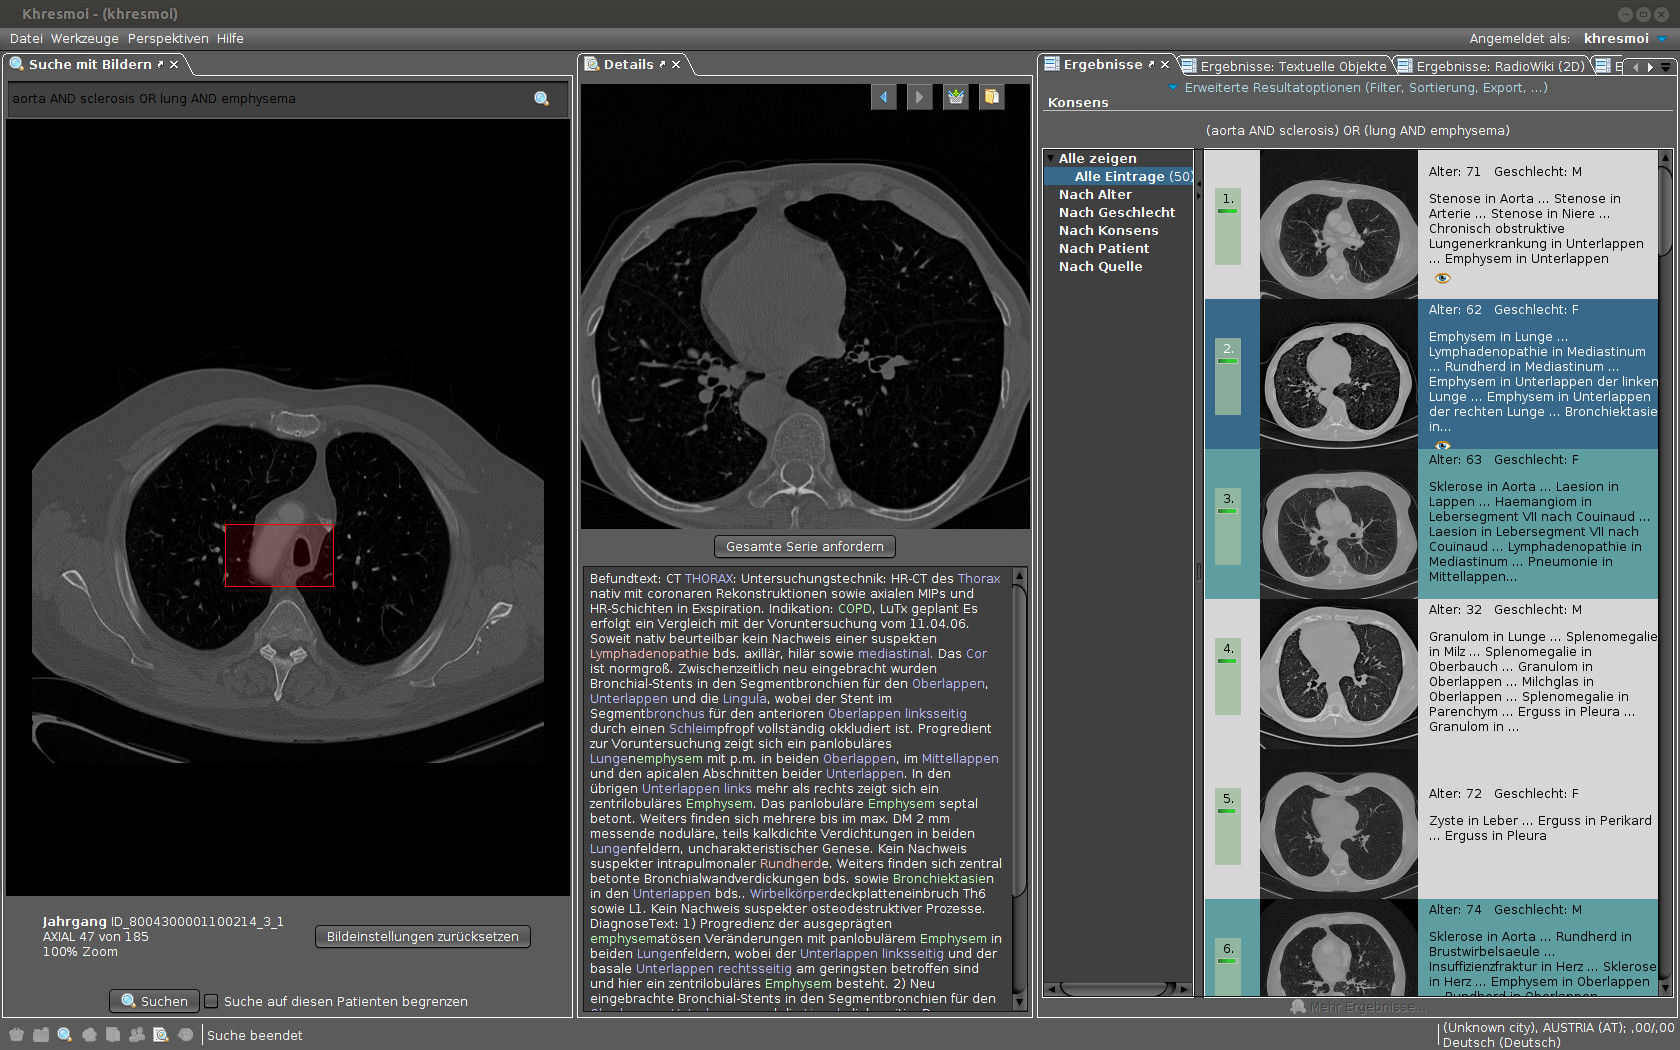
\includegraphics[width=\linewidth]{img/c4_java_client.jpg}
	\caption{JavaClient für KRESHMOI}
	\label{fig:java_client}
\end{figure}

\subsubsection{Layout}
\label{sec:ua_Layout}
Wie die Webapplikation wurde auch der JavaClient in mehrere Komponeten (Betrachter mit Suche, Ergebnisliste und Ergebnis Detailansicht) unterteilt.
Bei beiden können die Komponenten in dem Fenster unterschiedlich angeordnet und der Platz für die einzelnen Komponenten variiert werden.
Der JavaClient ist hierbei etwas dynamischer gestaltet da die Komponenten beliebig um positioniert werden können.
Weiters gibt es die Möglichkeit eine Komposition der Komponenten zu speichern.
Die Webapplikation verfügt über eine Menge von vordefinierten Kompositionen der Komponenten zwischen welchen gewechselt werden kann.

\subsubsection{Betrachter}
\label{sec:ua_Betrachter}
Beim Betrachter bieten beide Applikationen ungefähr den selben Funktionsumfang bzw. die selben Tools.
Ein wesentlicher Unterschied besteht in der Auswahl und Verwendung der Tools.
Die Webapplikation ist bei der Bedienung den zur zeit in der Medizin und Forschung verwendeten Programmen (Siehe Kapitel \ref{sec:relatedWork}) sehr ähnlich.
Bei diesen wird der Maus über eine Toolbar eine Aktion zugewiesen welche dann durch die Maustasten und Bewegen der Maus ausgeführt wird.
Der JavaClient hat ein eigenes Bedienkonzept welches von diesem Schema abweicht.
Bei diesem erfolgt der Wechsel zwischen den Tools durch die Maustasten, dem Drücken von Tasten am Keyboard und einem Kontextmenü.

\subsubsection{Ergebnissliste}
\label{sec:ua_Ergebnissliste}
Die Komponente zur Präsentation der Ergebnisse ist beim JavaClient um einiges Umfangreicher.
Dieser ermöglicht eine Ansicht der Ergebnisse als Tabelle von Bildern (wie in der Webapplikation) und als Liste welche auch eine Beschreibung und Bewertung der Datensätze enthält.
Weiters bietet er Funktionen um die Ergebnisse nach verschiedenen Kriterien zu sortieren und die Sucheregbnisse mit einer weiteren Textsuche einzuschränken.
Der JavaClient präsentiert auch Suchergebnisse aus anderen Ressourcen wie zu Beispiel aus einem Radiologie Wiki und ermöglicht eine Betrachtung dieser.
